\documentclass{article}
\usepackage[UTF8]{ctex}
\usepackage{geometry}
\usepackage{makecell}
\usepackage{amsmath}
\usepackage{graphicx}
\usepackage{subcaption}

\geometry{a4paper,scale=0.75}

\title{\heiti 实验十二\ 测定介质中声速}
\author{\kaishu 田睿轩\ 物理学院\ 1900011602}
\date{2020年12月3日}
\newcommand{\degree}{^\circ}
\newcommand{\degreesCelsius}{^\circ C}

\begin{document}
    \maketitle
    \section{实验数据与分析处理}
    \subsection{共振频率的测量}
    实验中,换能器发射端发射的声波经接收端反射,会在两者中间形成驻波,在刚性平面处,声压的振幅为:
    $$|p(l)|=\frac{\rho_0 \omega v a}{|\sin kl|}$$

    当$|\sin kl|$趋近于0时,声压的振幅会趋近于无穷,此时即形成共振。实际情况下声压振幅并不会趋于无穷,
    但会出现极大值。实验中,改变信号发生器的频率,并略微改变接收端的位置,使得接收端接收到的正弦波有最大振幅。
    此时信号发生器的频率即为共振频率$f_0$。

    实验中,测量得系统的共振频率$f_0$约$40.000kHz$,但为了波形能够具有较好的音色,方便之后利用极值法测量空气中声速,
    最后选定信号发生器的频率为$f_0=39.000kHz$。
   
    \subsection{极值法测量空气中声速}
    根据刚性平面处声压的振幅公式,当发射端与接收端之间的距离$l$改变,声压的振幅也会随之改变,
    当$l$的改变量为$\frac{\lambda}{2}$时,声压的振幅会复原(实际情况下,由于会有能量的损耗,因此并不会完全复原,但两次极大/小值之间$l$的变化量仍为$\frac{\lambda}{2}$)。
    实验中声压的振幅反映在示波器波形上,改变接收端的位置,记录下示波器波形每次出现极大的位置,两次极大之间接收端移动的距离即为半波长。

    实验中,分别增加发射端到接收端的距离,测量十次波形出现极大的位置并记录,实验数据如下所示:

    $f_0=39.000kHz$ \   $\theta = 19.1\degree C$
    \begin{center}
        \begin{tabular}{|c|c|c|c|c|c|c|c|c|c|c|}
            \hline
            $i$ & 0 & 1 & 2 & 3 & 4 & 5 & 6 & 7 & 8 & 9 \\
            \hline
            $x_i(mm)$ & 40.593 & 45.112 & 49.442 & 54.070 & 58.312 & 62.789 & 67.179 & 71.632 & 76.024 & 80.466 \\
            \hline 
            $U_{pp}(V)$  & 1.42 & 1.35 & 1.26 & 1.11 & 0.984 & 0.856 & 0.816 & 0.768 & 0.752 & 0.728 \\
            \hline
            $x_i^{'}(mm)$ & 80.361 & 75.831 & 71.376 & 66.926 & 62.530 & 58.138 & 53.963 & 49.262 & 44.839 & 40.333 \\
            \hline
            $U_{pp}^{'}(V)$ & 0.720 & 0.752 & 0.7668 & 0.824 & 0.880 & 1.01 & 1.12 & 1.27 & 1.34 & 1.43 \\
            \hline
        \end{tabular}
    \end{center}
    
    利用逐差法计算两次测量中声波的波长,再取平均作为空气中声波的波长。
    
    $$
    \begin{aligned}
        \frac{\lambda_2}{2}&=(\frac{x_0-x_5}{5}+\frac{x_1-x_6}{5}+\frac{x_2-x_7}{5}+\frac{x_3-x_8}{5}+\frac{x_4-x_9}{5})/5 \\
        &= (4.4392+4.4134+4.4380+4.3908+4.4308)/5 \\
        &= 4.4224 mm
    \end{aligned}
    $$

    $$
    \begin{aligned}
        \frac{\lambda_1}{2}&=(\frac{x_5-x_0}{5}+\frac{x_6-x_1}{5}+\frac{x_7-x_2}{5}+\frac{x_8-x_3}{5}+\frac{x_9-x_4}{5})/5 \\
        &= (4.4446+4.3936+4.4228+4.4174+4.4394)/5 \\
        &= 4.4236 mm
    \end{aligned}
    $$

    $$\frac{\lambda}{2}=(\frac{\lambda_1}{2}+\frac{\lambda_2}{2})/2=4.4230mm$$
    $$\lambda=8.8460mm$$
    $$v=\lambda f=345.00m/s$$

    下面计算该方法下声速的不确定度:
    $\sigma_v$由$\sigma_\lambda$和$\sigma_f$复合而成,因此,我们分别计算两者的不确定度
    
    实验中,最终计算出的$\frac{\lambda}{2}$可视为十个$\frac{\lambda_i}{2}$取平均,因此,用标准差来表征其不确定度,同时还要考虑仪器的允差。
    $\sigma_f$则直接用仪器的允差来表征。
    $$\sigma_1=\sqrt{\frac{\sum_{i=1}^{10} (N_i-\bar{N})^2}{n(n-1)}}=0.0061mm$$
    $$\sigma_{\frac{\lambda}{2}}=\sqrt{\sigma_1^2+(\frac{e}{\sqrt{3}})^2}=\sqrt{0.0061^2+(\frac{0.01}{\sqrt{3}})^2}=0.0084mm$$
    $$\sigma_\lambda=2\sigma_{\frac{\lambda}{2}}=0.017mm$$
    $$\sigma_f=\frac{e}{\sqrt{3}}=\frac{1}{\sqrt{3}}=0.58Hz$$
    $$\sigma_v=v\sqrt{(\frac{\sigma_\lambda}{\lambda})^2+(\frac{\sigma_f}{f})^2}=0.66m/s$$

    综上,得到极值法测空气中声速的结果为:
    $$v=(345.00\pm0.66)m/s$$

    \subsection{相位法测空气中声速}
    实验条件下,在发射端的声压和接收端的声压分别满足关系式:
    $$p(0)=-\rho_0 v \omega a \sin(\omega t)$$
    $$p(l)=-\rho_0 v \omega a \sin(\omega t-kl)$$

    即发射端和接收端的声压相位相差$kl$,可以通过示波器的XY模式观察李萨如图形来研究两者的相位差,
    当$l$变化$\lambda$时,相位差变化了$2\pi$,因此李萨如图形正好复原。实验中,移动接收端的位置,
    记录每次李萨如图形为右直线的位置,两相邻位置之间的差即为声波在空气中波长$\lambda$。

    实验数据如下表所示:
    
    $f_0=39.000kHz$\ $\theta=19.1\degreesCelsius$
    \begin{center}
        \begin{tabular}{|c|c|c|c|c|c|c|c|c|c|c|}
            \hline
            i & 0     & 1     & 2     & 3     & 4     & 5     & 6     & 7     & 8     & 9 \\
            \hline
            $x_i(mm) $ & 40.352  & 49.339  & 58.235  & 67.031  & 75.802  & 84.746  & 93.390  & 102.397  & 111.243  & 120.089  \\
            \hline
            $x_i^{'}(mm)$ & 120.580  & 110.908  & 102.212  & 93.248  & 84.395  & 75.450  & 67.692  & 57.872  & 49.111  & 40.140  \\
            \hline
        \end{tabular}
    \end{center}

    采用最小二乘法对数据进行处理,以i为横坐标,x为纵坐标进行线性拟合,由于横坐标i的间距恰好为1,
    所以直线的斜率的绝对值即为空气中声波波长$\lambda$,拟合后曲线如下所示:

    \begin{figure*}[h]
        \begin{center}
            \begin{subfigure}{0.48\textwidth}
                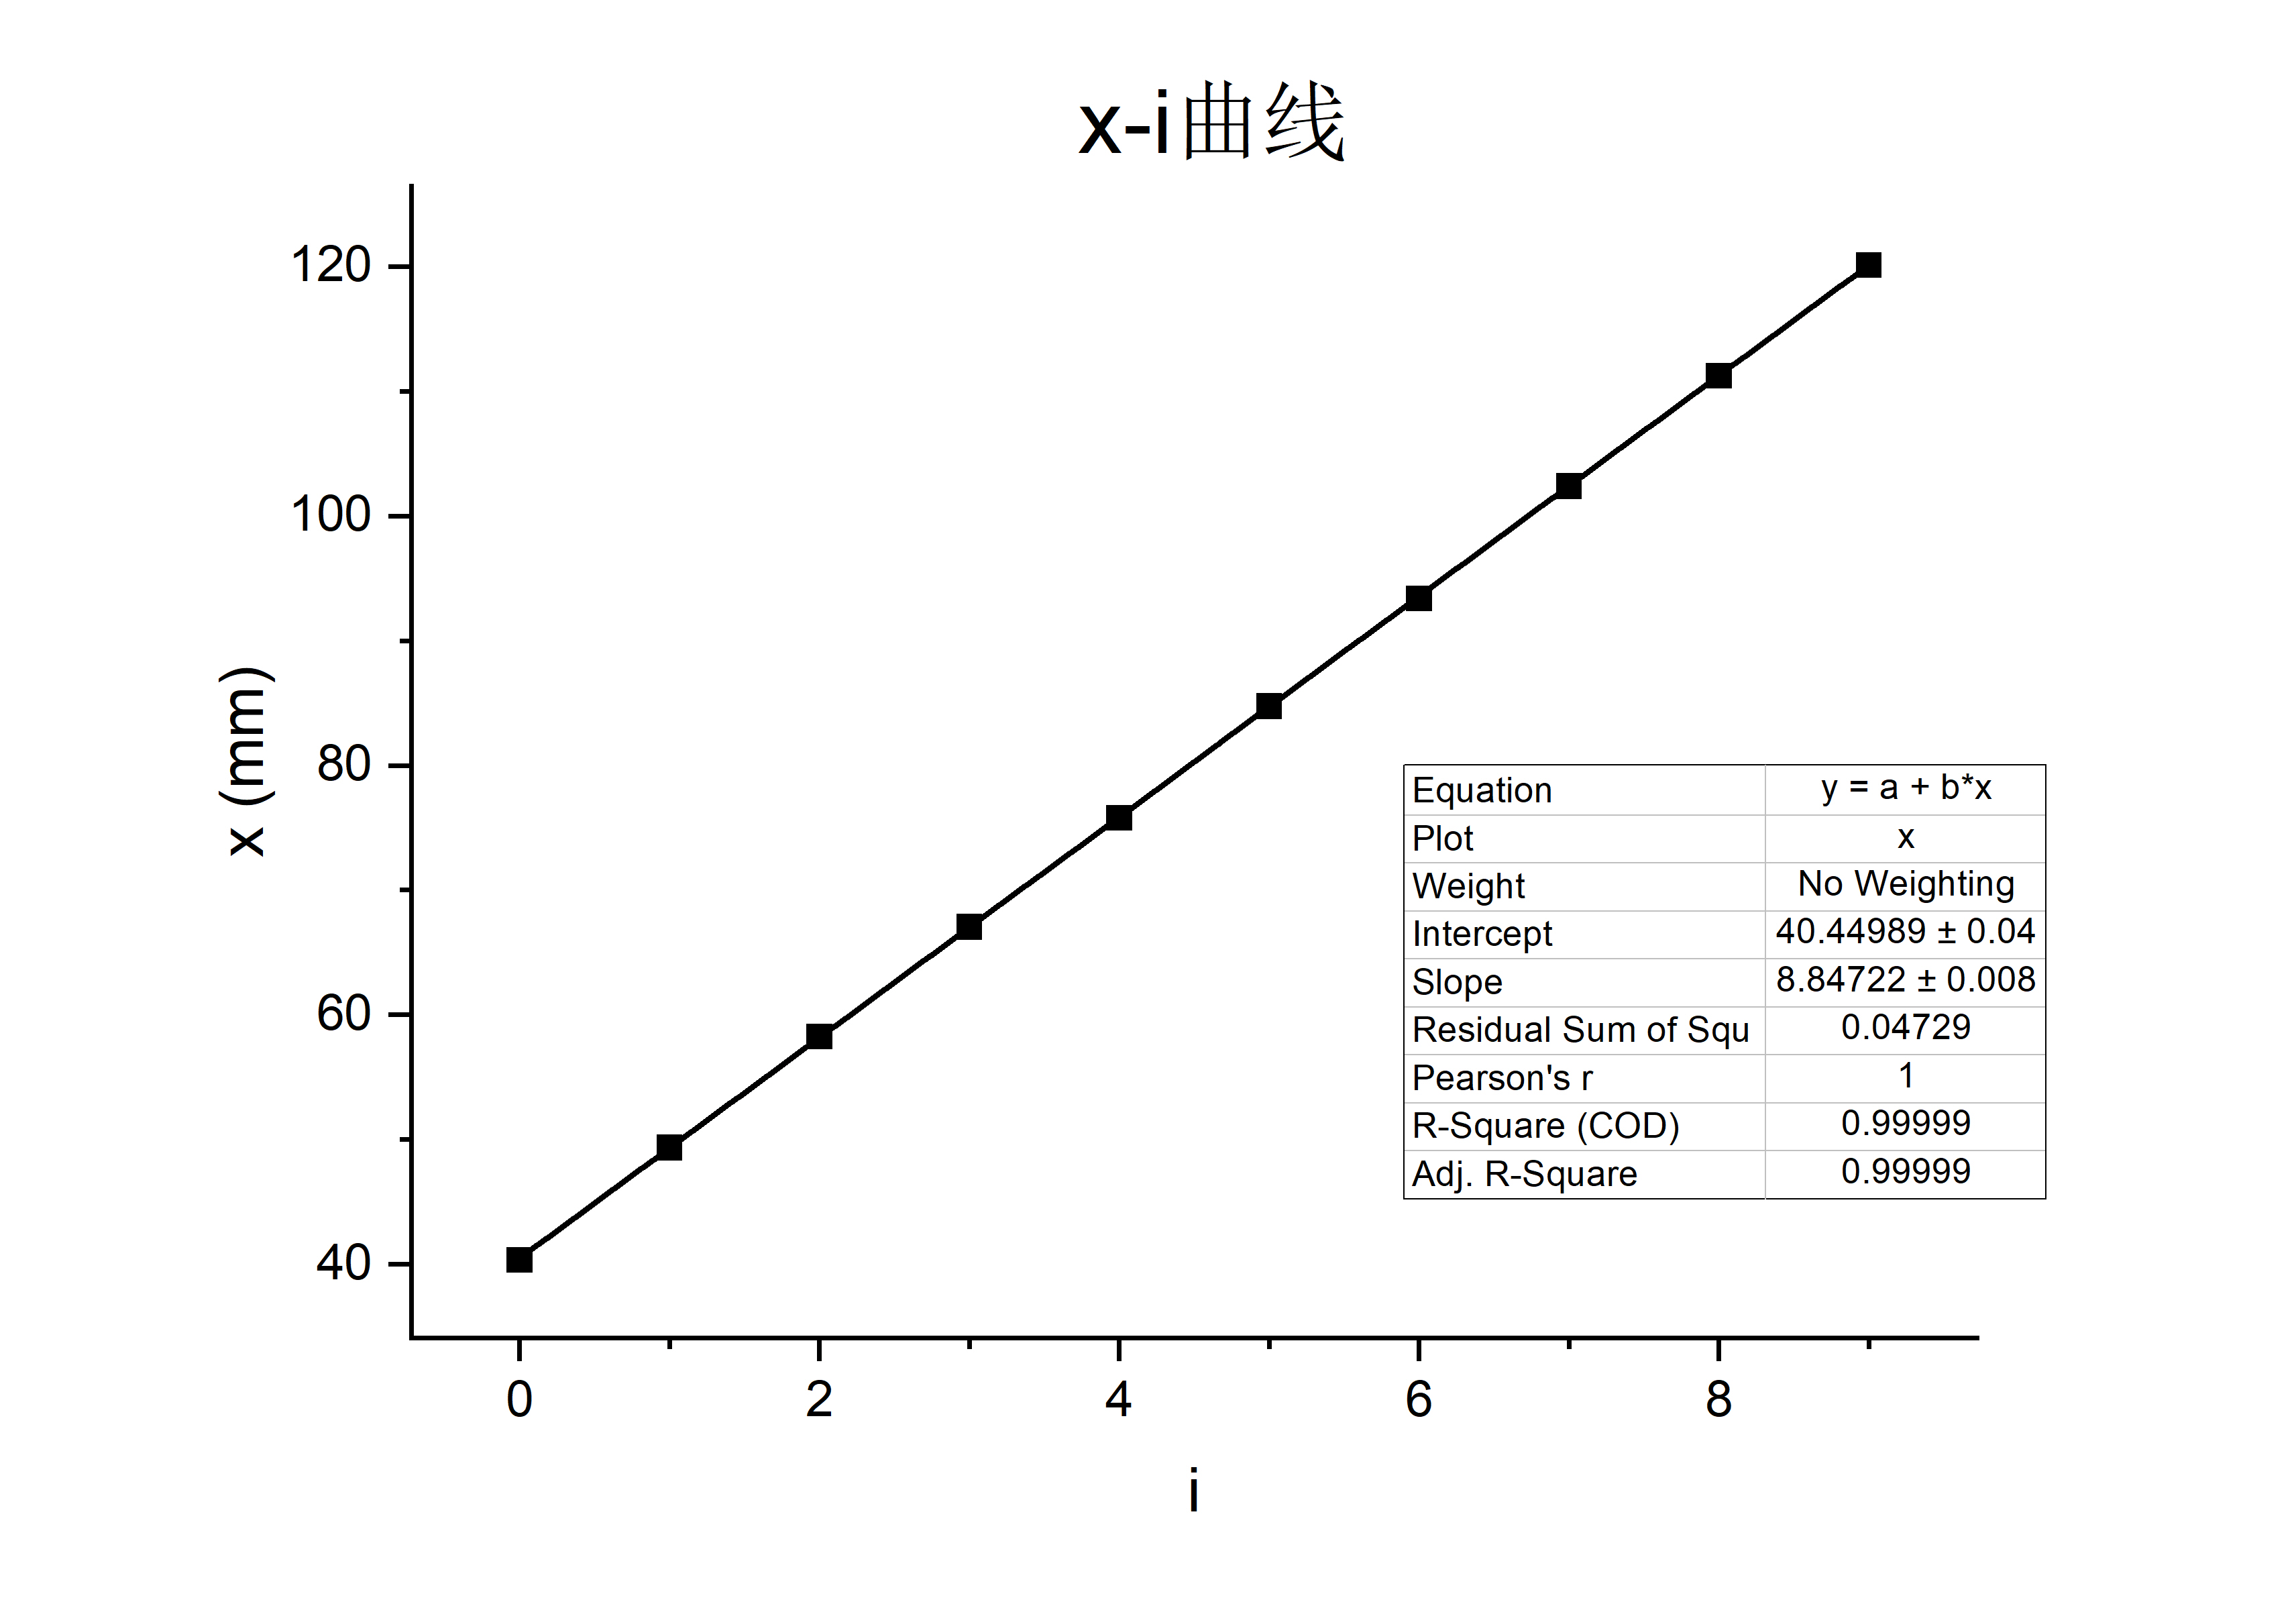
\includegraphics[width=\textwidth]{x-i curve.jpg}
            \end{subfigure}
            \begin{subfigure}{0.48\textwidth}
                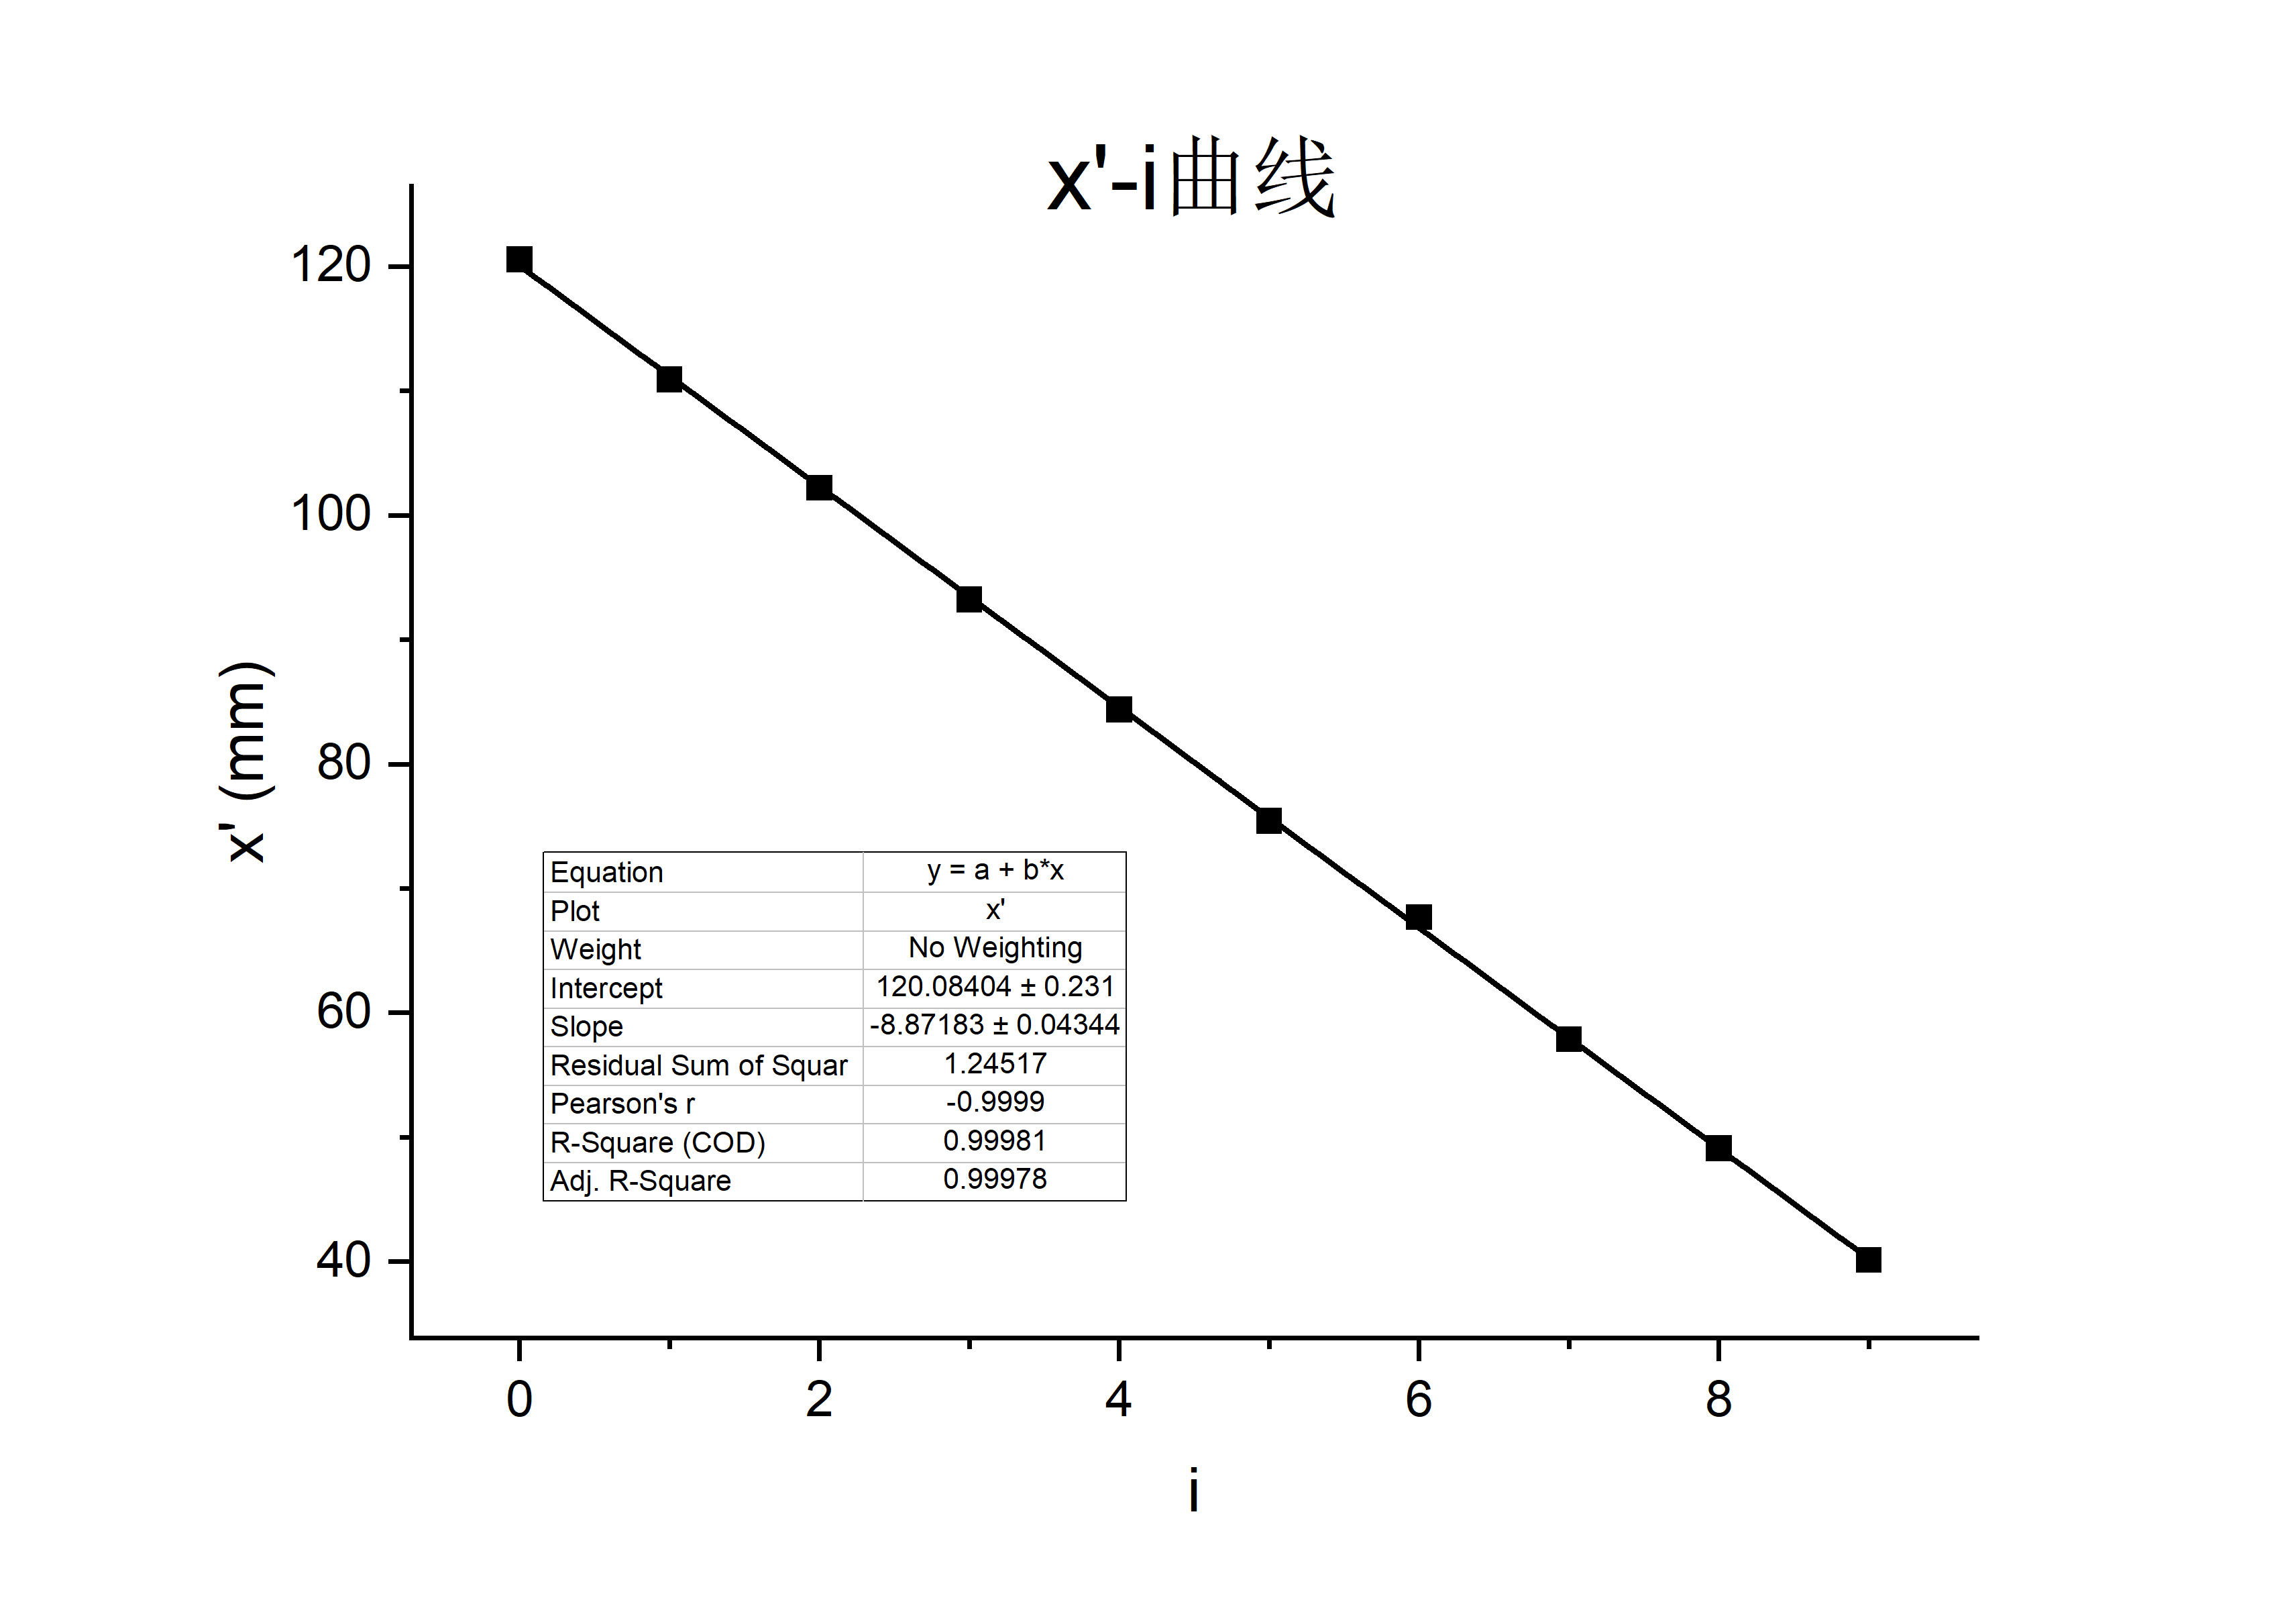
\includegraphics[width=\textwidth]{x'-i curve.jpg}
            \end{subfigure}
        \end{center}
    \end{figure*}

    由拟合数据可得:
    $$\lambda_1=8.8472mm,r_1=0.999996$$
    $$\lambda_2=8.8718mm,r_2=0.9999$$
    $$\lambda=\frac{\lambda_1+\lambda_2}{2}=8.8595mm$$
    $$v=\lambda f=345.52mm$$

    下面计算数据的不确定度:$\lambda$的不确定度由$\lambda_1$和$\lambda_2$的不确定度复合而成,
    其中两者的不确定度既包含拟合带来的A类不确定度,也包括仪器允差带来的B类不确定度:
    $$\sigma_{\lambda_1,A}=\lambda_1 \sqrt{\frac{1/r_1^2-1}{n-2}}=0.009mm$$
    $$\sigma_{\lambda_1,B}=\frac{\sigma_x}{\sqrt{\sum_{i=1}^n (x_i-\bar{x})^2}}=\frac{0.01/\sqrt{3}}{\sqrt{6457.1}}=7.2\times 10^{-5}mm$$
    $$\sigma_{\lambda_1}=\sqrt{(\sigma_{\lambda_1,A})^2+(\sigma_{\lambda_1,B})^2}=0.009mm$$
    $$\sigma_{\lambda_2,A}=\lambda_2 \sqrt{\frac{1/r_2^2-1}{n-2}}=0.044mm$$
    $$\sigma_{\lambda_2,B}=\frac{\sigma_x}{\sqrt{\sum_{i=1}^n (x'_i-\bar{x})^2}}=\frac{0.01/\sqrt{3}}{\sqrt{6494.8}}=7.2\times 10^{-5}mm$$
    $$\sigma_{\lambda_2}=\sqrt{(\sigma_{\lambda_2,A})^2+(\sigma_{\lambda_2,B})^2}=0.044mm$$
    $$\sigma_{\lambda}=\frac{1}{2}(\sigma_{\lambda_1}+\sigma_{\lambda_2})=0.026mm$$
    $$\sigma_v=v\sqrt{(\frac{\sigma_\lambda}{\lambda})^2+(\frac{\sigma_f}{f})^2}=1.01m/s$$

    综上,相位法测空气中声速的结果为:
    $$v=(345.52\pm1.01)m/s$$

    \subsection{气体参量法测空气中声速}
    若将空气视为绝热气体,且考虑空气中水蒸气的因素,则空气中声速可以用一下公式来计算:
    $$v=v_0\sqrt{(1+\frac{\theta}{T_0})(1+\frac{0.3192P_w}{P})}$$
    其中,$v_0=331.45m/s$为$\degreesCelsius$下空气中声速,$\theta$为摄氏温度,$T_0=273.15K$为
    $0\degreesCelsius$的绝对温度,$P_w=P_s H$为水蒸气分压,$P_s$为测量温度下的饱和蒸气压,$H$为湿度,
    $P$为大气压

    实验中测得的数据及各物理量的最小分度如下所示:
    
    \begin{center}
        \begin{tabular}{|c|c|c|c|c|}
            \hline
            & $\theta(\degreesCelsius)$ & $P_s(Pa)$ & $H(\%)$ & $P(mmHg)$\\
            \hline
            最小分度  & 1     & 0.1   & 2\%   & 0.05 \\
            \hline
            测量值   & 19.1  & 2211.0  & 36\%  & 775.50 \\
            \hline
        \end{tabular}
    \end{center}

    $$v=331.45\sqrt{(1+\frac{19.1}{273.15})(1+\frac{0.3192\times2211.0\times36\%}{775.50\times 133.3224})}=343.26m/s$$

    下面计算不确定度:
    $$\sigma_v=\sqrt{(\frac{\partial v}{\partial\theta}\sigma_\theta)^2 + (\frac{\partial v}{\partial P_S}\sigma_{P_S})^2+(\frac{\partial v}{\partial H}\sigma_H)^2+(\frac{\partial v}{\partial P}\sigma_P)^2}$$
    $$\frac{\partial v}{\partial\theta}\sigma_\theta=\frac{331.45^2(1+\frac{0.3192P_S H}{P\times133.3224}\frac{1}{T_0})}{2v}\sigma_\theta=0.34m/s$$
    $$\frac{\partial v}{\partial P_S}\sigma_{P_S}=\frac{331.25^2(1+\frac{\theta}{T_0})\frac{0.3192H}{P\times133.3224}}{2v}\sigma_{P_S}=1.1\times 10^{-5}m/s$$
    $$\frac{\partial v}{\partial H}\sigma_H=\frac{331.25^2(1+\frac{\theta}{T_0})\frac{0.3192P_S}{P\times133.3224}}{2v}\sigma_{H}=0.01m/s$$
    $$\frac{\partial v}{\partial P}\sigma_P=\frac{331.25^2(1+\frac{\theta}{T_0})\frac{0.3192P_S H}{P^2\times133.3224}}{2v}\sigma_{P}=0.003m/x$$
    $$\sigma_v=0.34m/s$$
    
    综上,得到气体参数法测量声速的结果:
    $$v=(343.26\pm0.34)m/s$$

    \subsection{能量随传播距离衰减规律}
    在极值法测空气中声速的实验中,声压振幅极大值处,波形的振幅可以用来表征接收端处在不同位置时能量的大小,
    可以用波形的电压峰峰值$U_{pp}$与$x$来的关系来研究声波随距离衰减规律

    \begin{center}
        \begin{tabular}{|c|c|c|c|c|c|c|c|c|c|c|}
            \hline
            $i$ & 0 & 1 & 2 & 3 & 4 & 5 & 6 & 7 & 8 & 9 \\
            \hline
            $x_i(mm)$ & 40.593 & 45.112 & 49.442 & 54.070 & 58.312 & 62.789 & 67.179 & 71.632 & 76.024 & 80.466 \\
            \hline 
            $U_{pp}(V)$  & 1.42 & 1.35 & 1.26 & 1.11 & 0.984 & 0.856 & 0.816 & 0.768 & 0.752 & 0.728 \\
            \hline
            $x_i^{'}(mm)$ & 80.361 & 75.831 & 71.376 & 66.926 & 62.530 & 58.138 & 53.963 & 49.262 & 44.839 & 40.333 \\
            \hline
            $U_{pp}^{'}(V)$ & 0.720 & 0.752 & 0.7668 & 0.824 & 0.880 & 1.01 & 1.12 & 1.27 & 1.34 & 1.43 \\
            \hline
        \end{tabular}
    \end{center}

    根据数据绘制曲线如下所示:

    \begin{figure*}[h]
        \begin{center}
            \begin{subfigure}[h]{0.48\textwidth}
                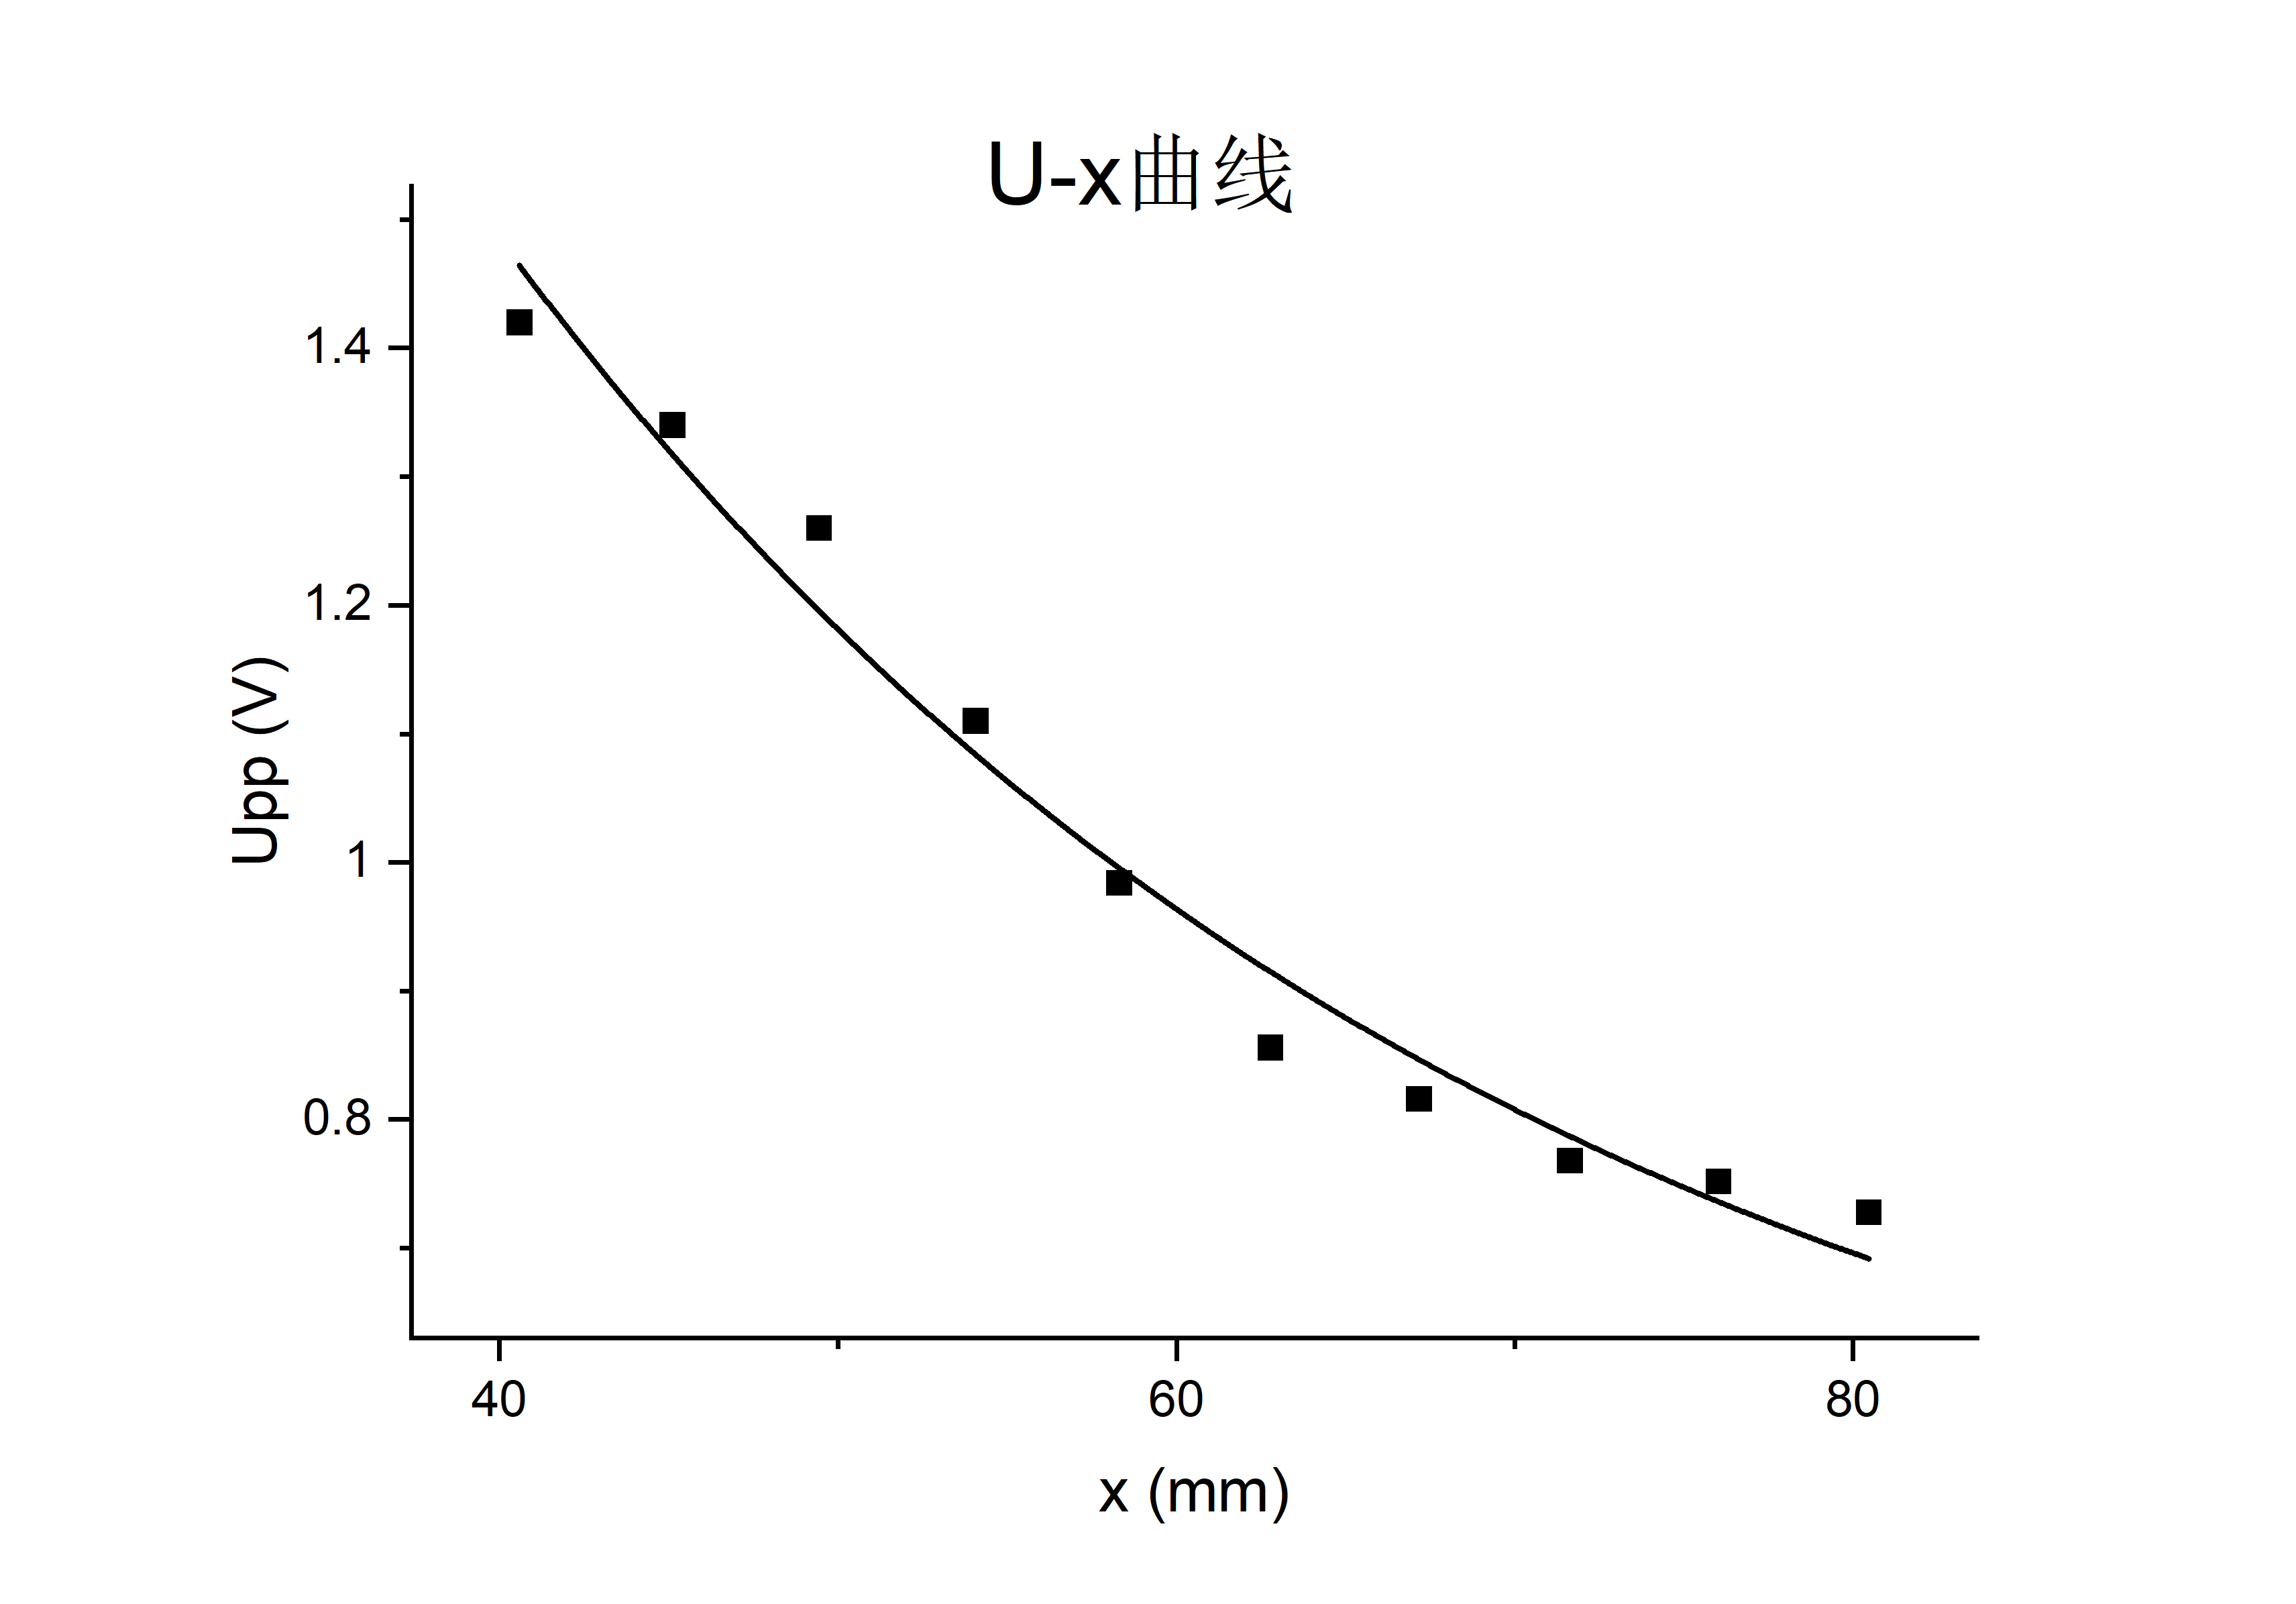
\includegraphics[width=\textwidth]{Upp-x curve.jpg}
            \end{subfigure}
            \begin{subfigure}[h]{0.48\textwidth}
                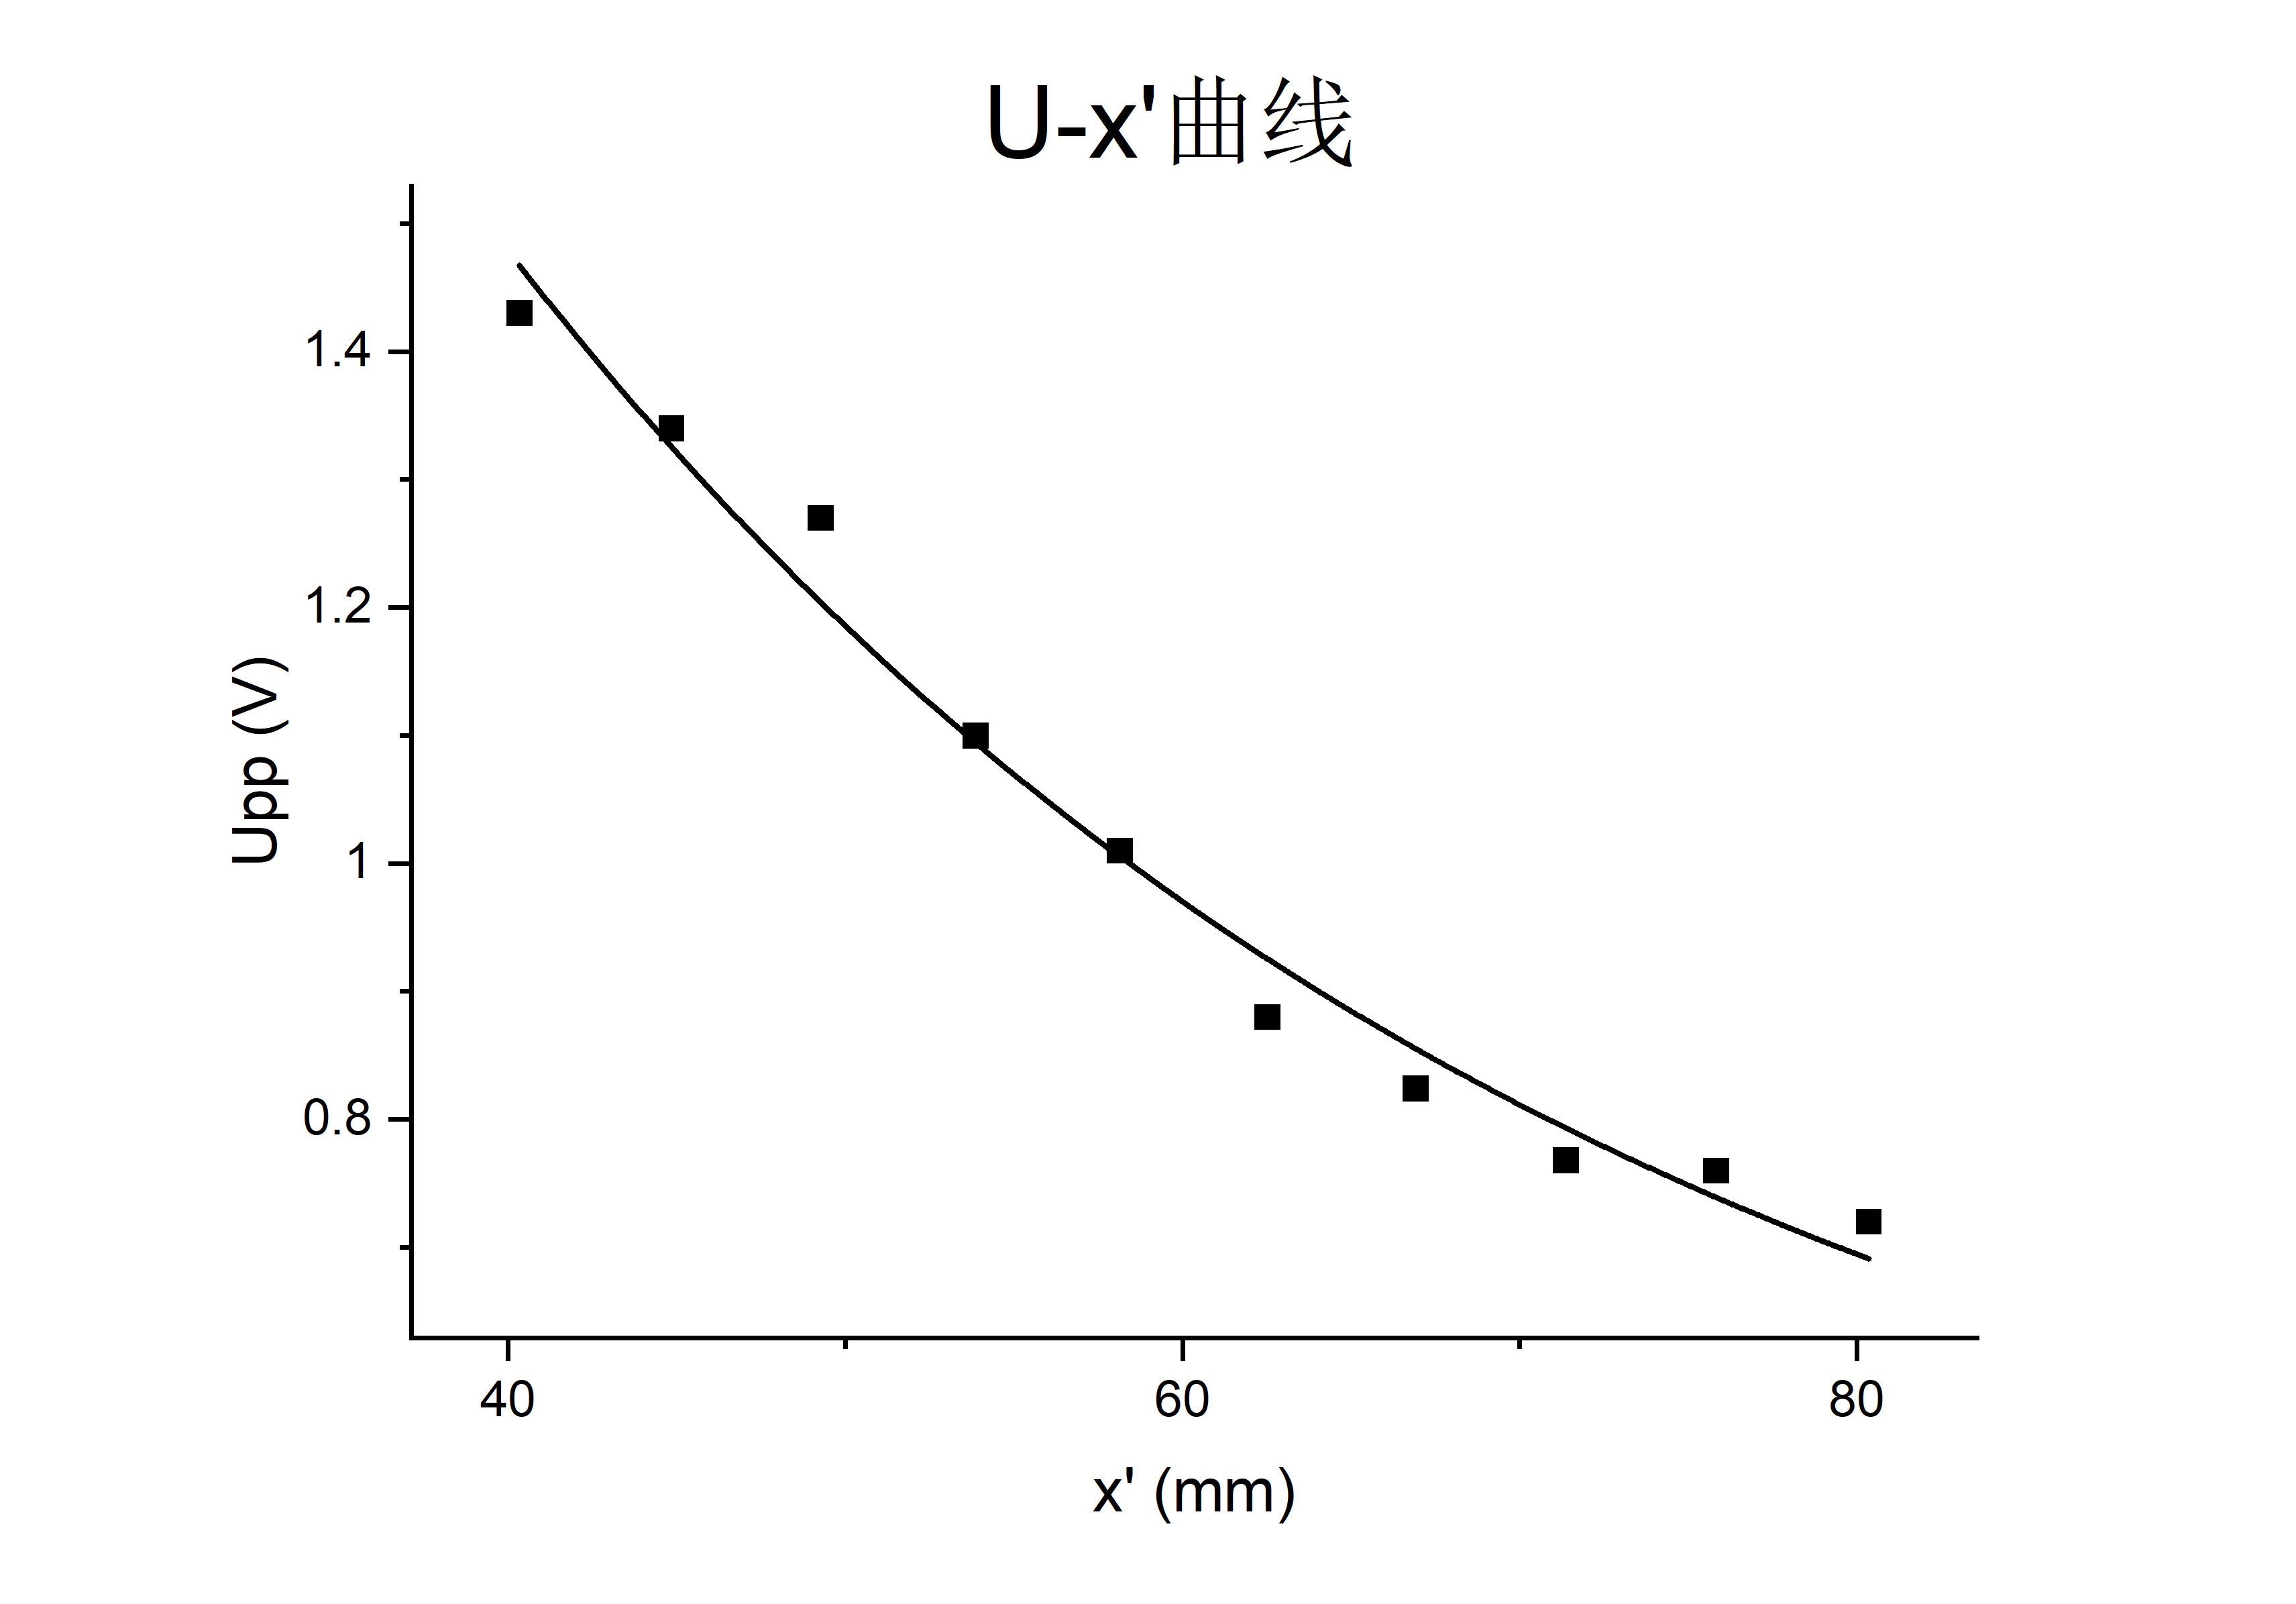
\includegraphics[width=\textwidth]{Upp-x' curve.jpg}
            \end{subfigure}
        \end{center}
    \end{figure*}

    $U_{pp}$随距离的关系基本满足指数衰减关系,说明能量随着距离的增加呈指数衰减。
    \subsection{超声光栅法测水中声速}
    当超声波在水中传播时,会形成疎密波,若光线垂直于声波传播方向入射,则会发生Ramann-Nath衍射,因此,
    超声波会在水中起到类似于光栅的作用,称为超声光栅,光栅常数$d$即为水中超声波的波长$\lambda$。
    $$\lambda=d=\frac{\lambda_{\text{光}}}{\sin \theta},\sin \theta \approx \tan \theta = \frac{x}{L}$$

    实验中,使用He-Ne激光器和透镜组构成光学系统,产生平行光。将超声换能器置于水中,平行光水平且垂直于声波方向入射,
    在远处产生衍射条纹。调节换能器的频率,使得衍射光的极强点最多,测量所需数据。

    \begin{center}
        \begin{tabular}{|c|c|c|c|c|}
            \hline
            $f(MHz)$ & $\lambda_{\text{光}}(nm)$ & $\theta_{\text{水}}(\degreesCelsius)$ & $x(cm)$ & $L(cm)$ \\
            \hline
            9.700 & 633 & 23.5 & 1.10 & 259.50 \\
            \hline
        \end{tabular}
    \end{center}

    $$\sin \theta \approx \tan \theta = \frac{x}{L}=4.24\times 10^{-3}$$
    $$\lambda=d=\frac{\lambda_{\text{光}}}{\sin \theta}=1.49\times 10^{-4}$$
    $$v=\lambda f=1448.5m/s$$

    \section{分析与讨论}
    \subsection{思考题}
    \subsubsection{误差来源}
    在极值法中,实验误差的一个主要来源是每次极大值点的判断,由于靠读示波器上的波形判断极大值点有一定难度,
    因此对每一次极大值点的位置不一定准确;而在相位法中,则是每一次李萨如图形回到相同图形时位置的标定,由于
    示波器上的图形本身有一定宽度且图线会抖动,很难使每次都显示为直线。这两种误差均为随机误差。
    \subsubsection{实验仪器和方法的改进}
    为了减小因位置标定不准确带来的误差,可以使用精度更高的示波器,在极值法中监测峰峰值,来辅助寻找极大值点。
    
    \section{实验收获}
    通过本次实验,我了解到了介质中测量声速的几种常用方法。此外,更加熟悉了示波器、信号发生器等常用仪器的使用。
    通过实验的过程和相关理论,对驻波、行波相关的知识有了进一步的认识。
\end{document}